%
% 04_komplexe_Integration.tex -- Auswertung des Umlaufzeit-Integrals
% mit komplexer Integration und Plausibilisierung des Resultats
%
% !TEX root = ../../buch.tex
% !TEX encoding = UTF-8
%
\section{Elliptische Bahnen und komplexe Integration
\label{kepler:section:komplex}}
\kopfrechts{Elliptische Bahnen und komplexe Integration}%

In diesem Abschnitt werten wir das Integral in \eqref{kepler:eqn:tintegral} für beliebige Exzentrizität $0<\varepsilon<1$ aus.
Dazu verwandeln wir das reelle Integral in ein Wegintegral über den komplexen Einheitskreis.
Diese Methode gehört zu den klassischen Anwendungen der Funktionentheorie \cite{kepler:freitagbusam}.
Eine unterhaltsame historische Einordnung findet sich bei Nahin \cite{kepler:nahin}.
Die Integrationsgrenzen $0$ und $2\pi$ sind der entscheidende Hinweis auf diese Methode.
Der Integrand hängt nur über $\cos(\vartheta)$ vom Winkel ab.
Er durchläuft also genau eine Periode.
Genauso durchläuft $e^{i\vartheta}$ genau einmal den Einheitskreis.

\subsection{Transformation auf den Einheitskreis
\label{kepler:subsection:substitution}}

Wir substituieren
\[
z
=
e^{i\vartheta}
\qquad\text{mit}\qquad
\cos(\vartheta)
=
\frac{e^{i\vartheta}+e^{-i\vartheta}}{2}
=
\frac12\biggl(z+\frac{1}{z}\biggr).
\]
Der Winkel $\vartheta$ läuft von $0$ bis $2\pi$.
Die Variable $z$ durchläuft dabei den Einheitskreis $C=\{z\in\mathbb{C}\mid |z|=1\}$ genau einmal im positiven Umlaufsinn.
Aus $dz=ie^{i\vartheta}\,d\vartheta$ folgt für das Differential
\[
d\vartheta
=
\frac{dz}{iz}.
\]
Vor dem Einsetzen bringen wir den Nenner des Integranden auf einen gemeinsamen Bruch:
\[
1+\varepsilon\cos(\vartheta)
=
1+\varepsilon\cdot\frac12\biggl(z+\frac{1}{z}\biggr)
=
\frac{\varepsilon z^2+2z+\varepsilon}{2z}.
\]
Damit wird aus dem reellen Integral das Wegintegral
\begin{align}
\int_0^{2\pi}
\frac{1}{(1+\varepsilon\cos(\vartheta))^2}
\,d\vartheta
&=
\oint_C
\frac{4z^2}{(\varepsilon z^2+2z+\varepsilon)^2}
\cdot
\frac{dz}{iz}
=
\frac{4}{i}
\oint_C
\frac{z}{(\varepsilon z^2+2z+\varepsilon)^2}
\,dz.
\notag
\intertext{Im Nenner klammern wir noch $\varepsilon^2$ aus.
So entsteht die Form}
%\int_0^{2\pi}
%\frac{1}{(1+\varepsilon\cos(\vartheta))^2}
%\,d\vartheta
&=
\frac{4}{i\varepsilon^2}
\oint_C
\frac{z}{\bigl(z^2+\frac{2}{\varepsilon}z+1\bigr)^2}
\,dz.
\label{kepler:eqn:wegintegral}
\end{align}
Mit ihr arbeiten wir im Folgenden.

\subsection{Lage der Polstellen
\label{kepler:subsection:polstellen}}

\begin{figure}
\centering
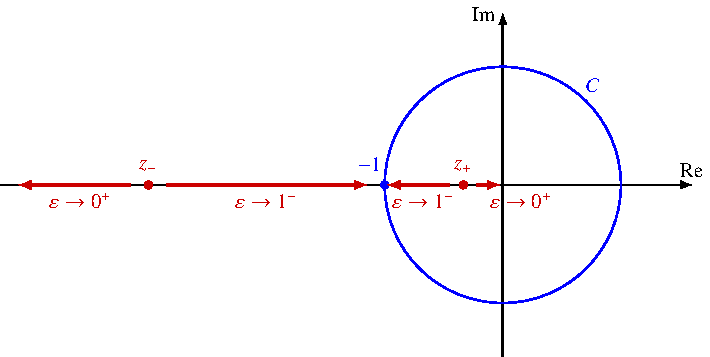
\includegraphics{papers/kepler/images/polstellen.pdf}
\caption{Lage der beiden Polstellen relativ zum Integrationsweg $C$.
Gezeichnet ist der Fall $\varepsilon=0.6$.
Beide Polstellen liegen auf der negativen reellen Achse, hier bei $z_+=-\frac13$ und $z_-=-3$.
Nur $z_+$ liegt im Inneren des Einheitskreises.
Nur dieser Pol trägt zum Wegintegral bei.
Die roten Pfeile deuten das Verhalten bei Veränderung von $\varepsilon$ an.
Für $\varepsilon\to 1^-$ streben beide Pole gegen den Punkt $-1$ auf dem Einheitskreis.
\label{kepler:figure:polstellen}}
\end{figure}


Der Wert eines Wegintegrals wird durch die Singularitäten im Inneren der Kurve bestimmt.
Wir suchen deshalb die Nullstellen des Nenners.
\index{Polstelle}%
Dazu lösen wir die quadratische Gleichung
\[
z^2+\frac{2}{\varepsilon}z+1
=
0
\qquad\Rightarrow\qquad
z_{\pm}
=
-\frac{1}{\varepsilon}\pm\!\sqrt{\frac{1}{\varepsilon^2}-1}.
\]
Wegen $0<\varepsilon<1$ ist der Radikand positiv.
Beide Nullstellen sind also reell und negativ.
Der Integrand hat in $z_+$ und $z_-$ je einen Pol zweiter Ordnung.
Auf dem Integrationsweg selbst liegen keine Pole.

Die Wurzelausdrücke sehen kompliziert aus.
Sie werden sich später aber stark vereinfachen.
Im Moment interessiert nur eine Frage: Welcher Pol liegt innerhalb von $C$?
Die Antwort auf diese Frage bekommen wir mittels Grenzwertbetrachtungen für $z_+$ und $z_-$.
Die roten Pfeile in Abbildung~\ref{kepler:figure:polstellen} zeigen, wie sich die beiden Pole dabei bewegen.

Für die Nullstelle $z_-$ gilt:
\begin{align*}
\lim_{\varepsilon \to 0^+} z_- &= \lim_{\varepsilon \to 0^+} \biggl(-\frac{1}{\varepsilon}-\!\sqrt{\frac{1}{\varepsilon^2}-1}\biggr) = -\infty, \\
\lim_{\varepsilon \to 1^-} z_- &= \lim_{\varepsilon \to 1^-} \biggl(-\frac{1}{\varepsilon}-\!\sqrt{\frac{1}{\varepsilon^2}-1}\biggr) = -1.
\end{align*}
Der Pol $z_-$ liegt also ausserhalb des Einheitskreises.

Für die Nullstelle $z_+$ verhalten sich die Grenzwerte folgendermassen:
\begin{align*}
\lim_{\varepsilon \to 0^+} z_+ &= \lim_{\varepsilon \to 0^+} \biggl(-\frac{1}{\varepsilon}+\!\sqrt{\frac{1}{\varepsilon^2}-1}\biggr) = 0, \\
\lim_{\varepsilon \to 1^-} z_+ &= \lim_{\varepsilon \to 1^-} \biggl(-\frac{1}{\varepsilon}+\!\sqrt{\frac{1}{\varepsilon^2}-1}\biggr) = -1.
\end{align*}
Wie wir sehen, liegt der Pol $z_+$ innerhalb des Einheitskreises.

Die Grenzwerte beschreiben allerdings nur die Ränder des Intervalls $0<\varepsilon<1$.
Den Nachweis für das ganze Intervall liefert der Satz von Vieta.
Nach ihm ist das Produkt der beiden Nullstellen $z_+z_-=1$.
Beide sind negativ, und wegen $z_-<z_+$ ist $|z_+|<|z_-|$.
Zusammen mit $|z_+|\,|z_-|=1$ folgt daraus $|z_+|<1<|z_-|$.
Für jede Exzentrizität $0<\varepsilon<1$ liegt also genau ein Pol im Inneren des Einheitskreises, nämlich $z_+$.

\subsection{Auswertung mit der Cauchy-Formel für Ableitungen
\label{kepler:subsection:cauchy}}

Wir wollen die Cauchy-Integralformel von
Satz~\ref{buch:integration:satz:residuensatz} anwenden, genauer ihre
Verallgemeinerung für Ableitungen.
Dazu schreiben wir den Integranden passend um.
Nur der Pol im Inneren soll noch explizit auftreten.
Mit den beiden Nullstellen $z_+$ und $z_-$ zerfällt der Nenner in die Linearfaktoren
\[
z^2+\frac{2}{\varepsilon}z+1
=
(z-z_+)(z-z_-).
\]
Damit ist
\begin{align}
\oint_C
\frac{z}{\bigl(z^2+\frac{2}{\varepsilon}z+1\bigr)^2}
\,dz
=
&
\oint_C
\frac{f(z)}{(z-z_+)^2}
\,dz
\qquad\text{mit}\qquad
f(z)
=
\frac{z}{(z-z_-)^2}.
\notag
\intertext{Die Funktion $f$ ist auf dem Einheitskreis und in seinem Inneren holomorph.
Ihre einzige Singularität $z_-$ liegt nämlich ausserhalb.
Der Pol in $z_+$ ist von zweiter Ordnung.
Wir brauchen deshalb die Cauchy-Formel für Ableitungen aus Satz~\ref{buch:integration:satz:ableitungn}.
\index{Cauchy-Integralformel}%
Für $n=1$ liefert sie}
&
\oint_C
\frac{f(z)}{(z-z_+)^2}
\,dz
=
2\pi i\,f'(z_+).
\label{kepler:eqn:ableitungsformel}
\end{align}
Das Wegintegral ist damit auf eine einzige Ableitung zurückgeführt.
\index{Wegintegral}%
Mit der Quotientenregel finden wir
\begin{align*}
f'(z)
&=
\frac{(z-z_-)^2-2z(z-z_-)}{(z-z_-)^4}
=
\frac{(z-z_-)-2z}{(z-z_-)^3}
=
-\frac{z+z_-}{(z-z_-)^3}.
\intertext{Jetzt setzen wir die Stelle $z_+$ ein.
Zähler und Nenner lassen sich direkt durch die Vieta-Beziehungen der quadratischen Gleichung $z^2+\smash{\frac{2}{\varepsilon}}z+1=0$ ausdrücken.
\index{Vieta-Beziehungen}%
Im Zähler steht die Summe $z_++z_-=-2/\varepsilon$.
Im Nenner steht die Differenz $z_+-z_-=2\smash{\sqrt{1/\varepsilon^2-1}}$.
Die unhandlichen Wurzelterme kombinieren sich dadurch zu}
f'(z_+)
&=
-\frac{z_++z_-}{(z_+-z_-)^3}
=
\frac{2/\varepsilon}{8\bigl(\frac{1}{\varepsilon^2}-1\bigr)^{\frac{3}{2}}}
=
\frac{1}{4\varepsilon}
\cdot
\biggl(\frac{\varepsilon^2}{1-\varepsilon^2}\biggr)^{\frac{3}{2}}
=
\frac{\varepsilon^2}{4\,(1-\varepsilon^2)^{\frac{3}{2}}}.
\end{align*}
Dieses Resultat setzen wir über \eqref{kepler:eqn:ableitungsformel}
in \eqref{kepler:eqn:wegintegral} ein.
Der Faktor $\varepsilon^2$ und die imaginäre Einheit heben sich weg.
Es bleibt der reelle Wert
\begin{equation}
\int_0^{2\pi}
\frac{1}{(1+\varepsilon\cos(\vartheta))^2}
\,d\vartheta
=
\frac{4}{i\varepsilon^2}
\cdot
2\pi i
\cdot
\frac{\varepsilon^2}{4\,(1-\varepsilon^2)^{\frac{3}{2}}}
=
\frac{2\pi}{(1-\varepsilon^2)^{\frac{3}{2}}}.
\label{kepler:eqn:integralwert}
\end{equation}
Am Ende kommt also eine reelle Zahl heraus.
Das ist eine willkommene Kontrolle, denn das Ausgangsintegral war reell.
Auch der Grenzfall stimmt.
Für $\varepsilon\to 0$ liefert \eqref{kepler:eqn:integralwert} den Wert $2\pi$.
Denselben Wert haben wir in
Abschnitt~\ref{kepler:subsection:integralspezialfall} für die
Kreisbahn direkt berechnet.

\subsection{Das dritte keplersche Gesetz
\label{kepler:subsection:resultat}}

Jetzt setzen wir alles zusammen.
Mit dem Integralwert \eqref{kepler:eqn:integralwert} wird aus der
Umlaufzeit \eqref{kepler:eqn:tintegral}
\begin{align}
T
&=
\frac{m\,p^2}{L}
\cdot
\frac{2\pi}{(1-\varepsilon^2)^{\frac{3}{2}}}.
\notag
\intertext{Den Drehimpuls ersetzen wir mit
\eqref{kepler:eqn:drehimpulsgeometrie} durch $L=m\sqrt{GMp\mathstrut}$.
Die Planetenmasse $m$ kürzt sich dabei wie schon im Kreisfall heraus:}
T
&=
\frac{p^2}{\!\sqrt{GMp\mathstrut}}
\cdot
\frac{2\pi}{(1-\varepsilon^2)^{\frac{3}{2}}}
=
\frac{2\pi}{\!\sqrt{GM\mathstrut\rlap{$\phantom{p}$}}}
\cdot
\frac{p^{\frac{3}{2}}}{(1-\varepsilon^2)^{\frac{3}{2}}}.
\notag
\intertext{Nach \eqref{kepler:eqn:ellipse} ist $p=a(1-\varepsilon^2)$.
Der Faktor $(1-\varepsilon^2)$ fällt damit vollständig aus der Formel heraus:}
T
&=
\frac{2\pi}{\!\sqrt{GM\mathstrut\rlap{$\phantom{p}$}}}
\cdot
\frac{a^{\frac{3}{2}}(1-\varepsilon^2)^{\frac{3}{2}}}{(1-\varepsilon^2)^{\frac{3}{2}}}
=
\frac{2\pi\,a^{\frac{3}{2}}}{\!\sqrt{GM\mathstrut\rlap{$\phantom{p}$}}}.
\notag
\intertext{Die Umlaufzeit hängt also weder von der Masse des Planeten noch von der Exzentrizität seiner Bahn ab.
Sie hängt nur von der grossen Halbachse und der Masse des Zentralgestirns ab.
Quadrieren liefert das dritte keplersche Gesetz in seiner üblichen Form
\index{keplersches Gesetz!drittes}}
\frac{T^2}{a^3}
&=
\frac{4\pi^2}{GM}
=
\text{konstant}.
\label{kepler:eqn:keplerdrei}
\end{align}
Für $\varepsilon=0$ und $a=r$ enthält es das Resultat
\eqref{kepler:eqn:kreisbahn} für Kreisbahnen als Spezialfall.

\subsection{Plausibilisierung anhand realer Bahndaten
\label{kepler:subsection:plausibilisierung}}

\begin{table}
\centering
\begin{tabular}{lrrrr}
Körper & $\varepsilon$ & $a$ in $\text{m}$ & $T$ in $\text{s}$
& $T^2/a^3$ in $\text{s}^2\text{m}^{-3}$
\\
\hline
Erde   & $0.017$ & $1.496\cdot 10^{11}$ & $3.156\cdot 10^{7}$
& $2.975\cdot 10^{-19}$
\\
Mars   & $0.094$ & $2.279\cdot 10^{11}$ & $5.935\cdot 10^{7}$
& $2.976\cdot 10^{-19}$
\\
67P    & $0.641$ & $5.180\cdot 10^{11}$ & $2.033\cdot 10^{8}$
& $2.974\cdot 10^{-19}$
\end{tabular}
\caption{Bahndaten der Erde, des Mars und des Kometen
67P/Tschurjumow-Gerassimenko nach \cite{kepler:nasafactsheet} und
\index{Erde}%
\index{Mars}%
\index{67P/Tschurjumow-Gerassimenko}%
\index{Tschurjumow-Gerassimenko}%
\cite{kepler:jplsbdb}.
Die Exzentrizitäten $\varepsilon$ der drei Körper sind sehr unterschiedlich.
Trotzdem stimmt der Quotient $T^2/a^3$ überall auf drei Stellen mit
dem theoretischen Wert
$4\pi^2/GM_{\odot}=2.975\cdot 10^{-19}\,\text{s}^2\text{m}^{-3}$
überein.
\label{kepler:table:plausibilisierung}}
\end{table}

Zum Schluss prüfen wir das Resultat \eqref{kepler:eqn:keplerdrei} an realen Daten.
Tabelle~\ref{kepler:table:plausibilisierung} vergleicht die Erde, den Mars und den Kometen 67P/Tschurjumow-Gerassimenko.
Der Komet ist durch die Rosetta-Mission bekannt geworden.
Als Testfall ist er besonders interessant.
Seine Bahn hat die Exzentrizität $\varepsilon\approx 0.641$.
Sie ist damit weit von einer Kreisbahn entfernt.
Die Kreisbahn-Herleitung aus Abschnitt~\ref{kepler:subsection:kraeftegleichgewicht} macht über ihn deshalb keine Aussage.
Die Bahndaten stammen aus \cite{kepler:nasafactsheet} und \cite{kepler:jplsbdb}.
Für die Sonne gilt $GM_{\odot}=1.327\cdot 10^{20}\,\text{m}^3\text{s}^{-2}$.
Damit ergibt sich für alle drei Körper derselbe Quotient $T^2/a^3$.
Er stimmt mit dem theoretischen Wert $4\pi^2/GM_{\odot}$ überein.

Das dritte keplersche Gesetz ist damit für beliebige elliptische Bahnen bewiesen und numerisch bestätigt.
Die Unabhängigkeit von der Planetenmasse macht es zu einem praktischen Werkzeug.
Man misst die Umlaufzeit und die Halbachse eines einzigen Begleiters.
Daraus liefert \eqref{kepler:eqn:keplerdrei} die Masse des Zentralkörpers.
So bestimmt man die Masse der Sonne, eines Planeten mit Monden oder eines fernen Sterns mit Exoplaneten.
Aus Sicht dieses Seminars ist vor allem der Weg bemerkenswert.
Am Anfang stand ein reelles Integral, an dem sich die Schulanalysis die Zähne ausbeisst.
In der komplexen Ebene zerfiel es in drei einfache Schritte: eine Substitution, eine quadratische Gleichung und eine einzige Ableitung.
